\lhead{\emph{Motivación y objetivos}}
\chapter{Motivación y objetivos}

El presente proyecto responde al interés personal en las áreas de conocimiento relacionadas con la Computación Distribuida. La propuesta final cuenta con un atractivo añadido, que es la utilización de computadores embebidos, generalmente no utilizados para este tipo de propósitos, como integrantes de un sistema distribuido. En diferentes reuniones entre las diferentes partes se terminan de perfilar los diferentes objetivos a completar, entre los que destaca la potencial integración del sistema en asignaturas del plan de estudios del Grado en Ingeniería Informática como herramienta didáctica.

\section{Objetivos}

El sistema creado se inspira en proyectos similares y se diseña con el objetivo de dar solución a diferentes necesidades identificadas como estudiante de varias asignaturas del currículo del Grado en Ingeniería Informática. El sistema cuenta con cuatro objetivos a alto nivel independientes:

\begin{itemize}
	\item Como síntesis de los conocimientos adquiridos en la carrera, se busca la creación de un sistema completo desde sus cimientos hasta los componentes de más alto nivel, gestionando las tareas de mantenimiento, instalación y manejo del mismo, así como los protocolos de trabajo, tanto en cada uno de los componentes del sistema como en la comunicación entre los mismos. Con un enfoque más teórico, se pretende crear un sistema capaz de poder ser utilizado como herramienta de diseño y prueba de algoritmos que resuelvan problemas aprovechando la distribución de tareas, así como el análisis de dichos algoritmos utilizando versiones finales del sistema.

	\item Potenciar su uso como herramienta de aprendizaje en las áreas de conocimiento Sistemas Operativos, Algoritmia, Redes de Computadores, Sistemas Distribuidos, Administración de Sistemas y Sistemas Embebidos.
	
	\item Constituir una herramienta didáctica para varias asignaturas del currículo del Grado en Ingeniería Informática de la Universidad de Salamanca, analizando aquellas relevantes y proponiendo soluciones a las diferentes necesidades propuestas por el Profesorado, Estudiantes y Administradores del sistema, en colaboración con dichas partes.

	\item Intentar elevar el \textit{state of the art} en el mundo de los sistemas distribuidos con plataformas embebidas mediante la creación de un sistema multipropósito en lugar de soluciones con un fin determinado, que constituyen la tendencia actual.
\end{itemize}


Partiendo de la premisa de las potenciales ventajas del uso de este tipo de computadores en detrimento de otras soluciones se plantea el sistema definitivo (en \ref{alternativas} se detalla el proceso de decisión), no sin antes realizar una etapa de evaluación de las diferentes alternativas.

\section{Objetivos del sistema}

Durante las fases de definición del proyecto, se plantean los siguientes objetivos concretos para la propuesta de solución elegida que se deben cumplir:

\subsection{Diseño y construcción de la arquitectura física del sistema}

Se deberán definir las interconexiones entre los diferentes componentes del sistema, solucionar los diferentes problemas físicos tales como la alimentación eléctrica, conexiones de red o la refrigeración, entre otros, analizando los diferentes enfoques y valorando la mejor solución en función del resto de objetivos a cumplir.

\subsection{Arquitectura orientada a servicios}
%TODO
Conjunto de servicios que podrán ser aprovechados por diferentes clientes para explotar la capacidad de cálculo de las máquinas.

\subsection{Gestión del sistema}

El sistema debe contar con un conjunto de herramientas que mantengan los principios de transparencia propios de un sistema distribuido (ver \ref{transparencia}), y su gestión debe ser sencilla para los responsables del mismo (personal de administración).

\subsection{Integración}

El sistema debe integrarse en una infraestructura preexistente, la presente en la Facultad de Ciencias de la Universidad de Salamanca, sin que dicha integración comprometa el diseño básico del sistema a fin de facilitar su adaptabilidad a otros entornos (ver \ref{infraestructura}). Es necesario por tanto realizar pruebas que evalúen el rendimiento del sistema creado en la misma. %TODO Con el objetivo de facilitar dicha integración, el sistema se desarrolla parcialmente aprovechando la infraestructura presente.

\subsection{Uso como herramienta didáctica}

El sistema debe ofrecer una serie de ventajas a las herramientas didácticas utilizadas en aquellas asignaturas donde se impartan conocimientos relacionados con la computación paralela y distribuida, ofreciendo herramientas que faciliten la comprensión de dichos paradigmas o el desarrollo, prueba y aplicación de programas basados en los mismos.

%TODO: Creación de aplicaciones, herramientas y documentación como alternativa a las instalaciones típicas utilizadas actualmente.

\subsection{Evaluación}

A fin de probar los objetivos definidos anteriormente, la viabilidad de sistema como herramienta didáctica y su integración en la organización deberán ser determinados por los diferentes usuarios de la misma y la realización de pruebas de integración.

Durante el desarrollo del proyecto se añaden los siguientes objetivos funcionales:

%TODO Incluir en los objetivos de MarcoPolo
\subsection{Simplicidad de MarcoPolo}

MarcoPolo debe conseguir un alto grado de versatilidad y aplicabilidad en un gran rango de aplicaciones. A fin de conseguir este objetivo, la simplicidad del sistema construido es clave. Esto conlleva el desacoplamiento y delegación de gran parte de la funcionalidad a otras capas superiores, independientes del protocolo, pero que aprovechan su funcionalidad, en lugar de ser integradas en el mismo (ver \ref{marcopolo}).

\subsection{Test-Driven Development}

El desarrollo de las diferentes herramientas \textit{software} se deberá realizar bajo los principios del desarrollo conducido por pruebas (ver \ref{tdd}) como mecanismo para la detección temprana de errores.

\chapter{Situación actual (\textit{state of the art})}
\lhead{Situación actual (\textit{state of the art})}

En esta sección se definen diferentes enfoques ya aplicados a soluciones a problemas similares al planteado anteriormente.

\section{Computadores de placa única}

El uso de computadores de prestaciones reducidas como componentes de un sistema distribuido ha experimentado un gran crecimiento en los últimos años debido a la popularización y el abaratamiento de este tipo de dispositivos, existiendo gran cantidad de fabricantes y proveedores de \textit{software} para los mismos.

Los computadores de placa única (\textit{Single-Board Computers}) son máquinas de generalmente bajas prestaciones que aglutinan todos los componentes necesarios para su funcionamiento en un único circuito impreso. Suelen tener un coste bajo y una relación rendimiento/coste elevada. Su versatilidad y precio reducido han propiciado su uso como herramienta para el estudio y creación de sistemas distribuidos con un gran rango de propósitos diferentes.

\subsection{RPiCluster (Joshua Kiepert)}

Joshua Kiepert, estudiante de doctorado en la universidad Boise State, crea este sistema utilizando 33 computadores \textbf{Raspberry Pi B}, con el objetivo de utilizarlo como herramienta de pruebas que sirva de alternativa al supercomputador con el que su universidad cuenta\cite{joshuarpicluster} y sobre el que trabaja de forma rutinaria, con el objetivo de poder continuar su trabajo en periodos de mantenimiento, cierre del centro, etcétera. El sistema está diseñado para utilizar la \textit{Message Passing Interface} como mecanismo de comunicación y coordinación (siguiendo un esquema maestro-esclavo) y además utilizar los diferentes puertos de las placas (GPIO, I\textsuperscript{2}C, SPI, UART), puertos generalmente ausentes en computadores convencionales. Utiliza además un sistema \textbf{NFS} (\textit{Network File Storage}) para compartir datos entre todos los nodos, y un \textit{router} dedicado para la interconexión. El sistema se completa con un ordenador portátil \textbf{Chromebook} con el mismo sistema operativo que los nodos del sistema, (\textbf{Arch Linux}), que actúa como nodo coordinador. La estructura incluye el conjunto de nodos esclavos y coordinador, dos fuentes de alimentación y un mecanismo de refrigeración, así como un mecanismo de distribución de la energía (diseñado por Kiepert) y de gestión de los diodos LED que incluye cada nodo y que son utilizados como elemento estético y mecanismo de análisis visual del comportamiento de los algoritmos ejecutados\footnote{Vídeo del sistema en ejecución: \href{https://www.youtube.com/watch?v=i_r3z1jYHAc}{youtube.com/watch?v=i\_r3z1jYHAc}}.

%TODO: http://www.zdnet.com/article/build-your-own-supercomputer-out-of-raspberry-pi-boards/

\begin{figure}[H]
	\centering
	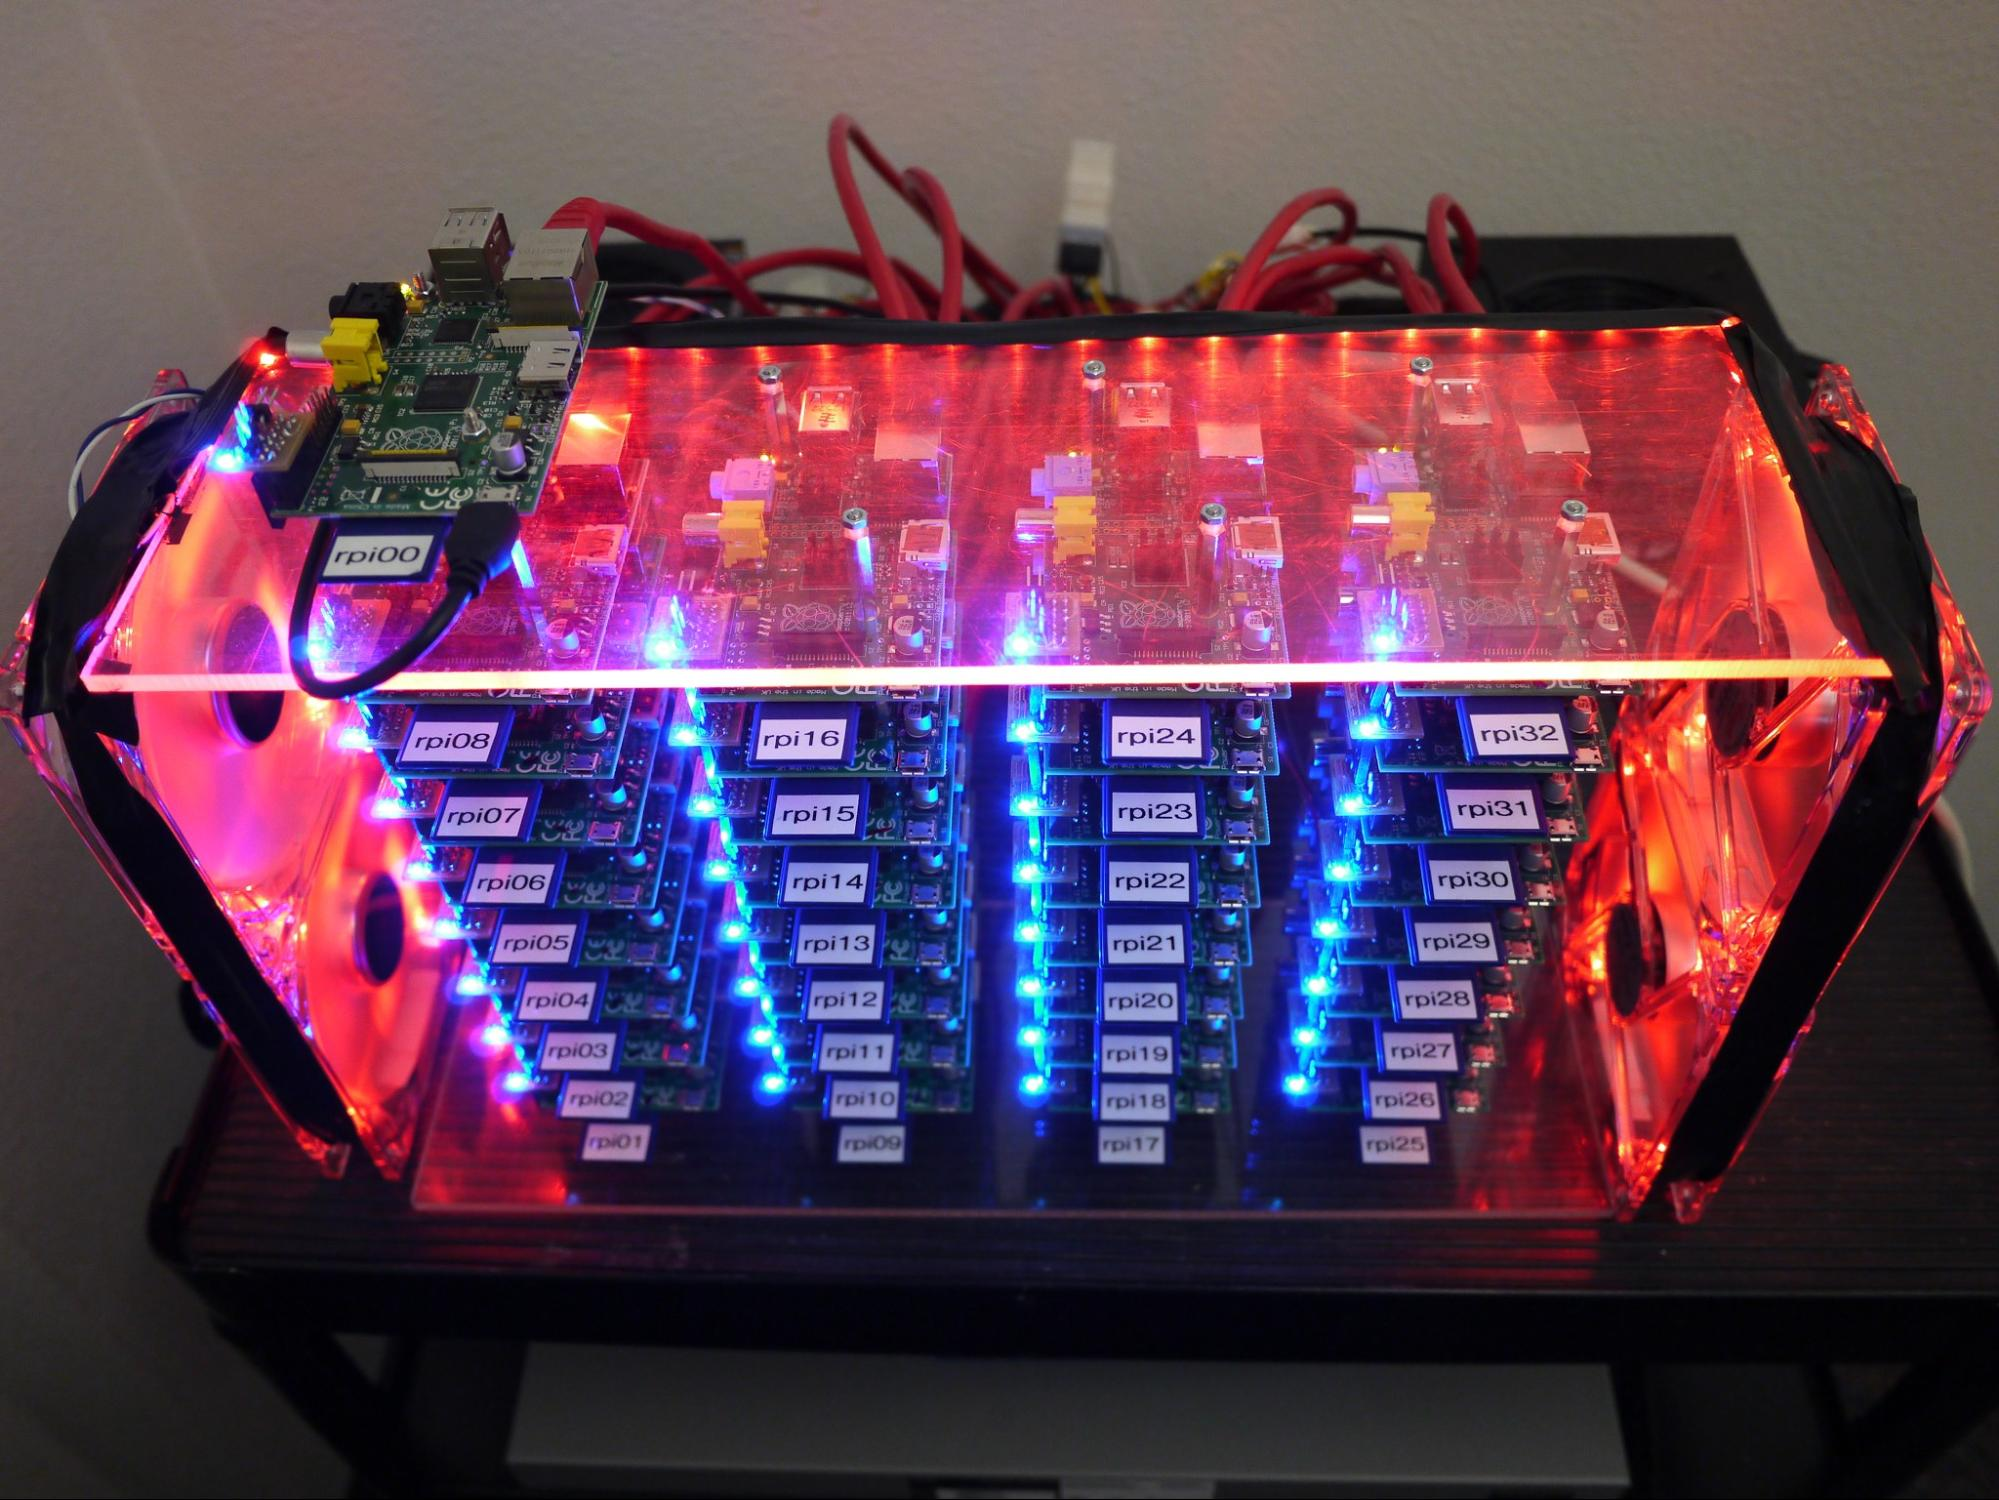
\includegraphics[width=0.36\textwidth]{Chapter1/Figures/kiepert-main}
	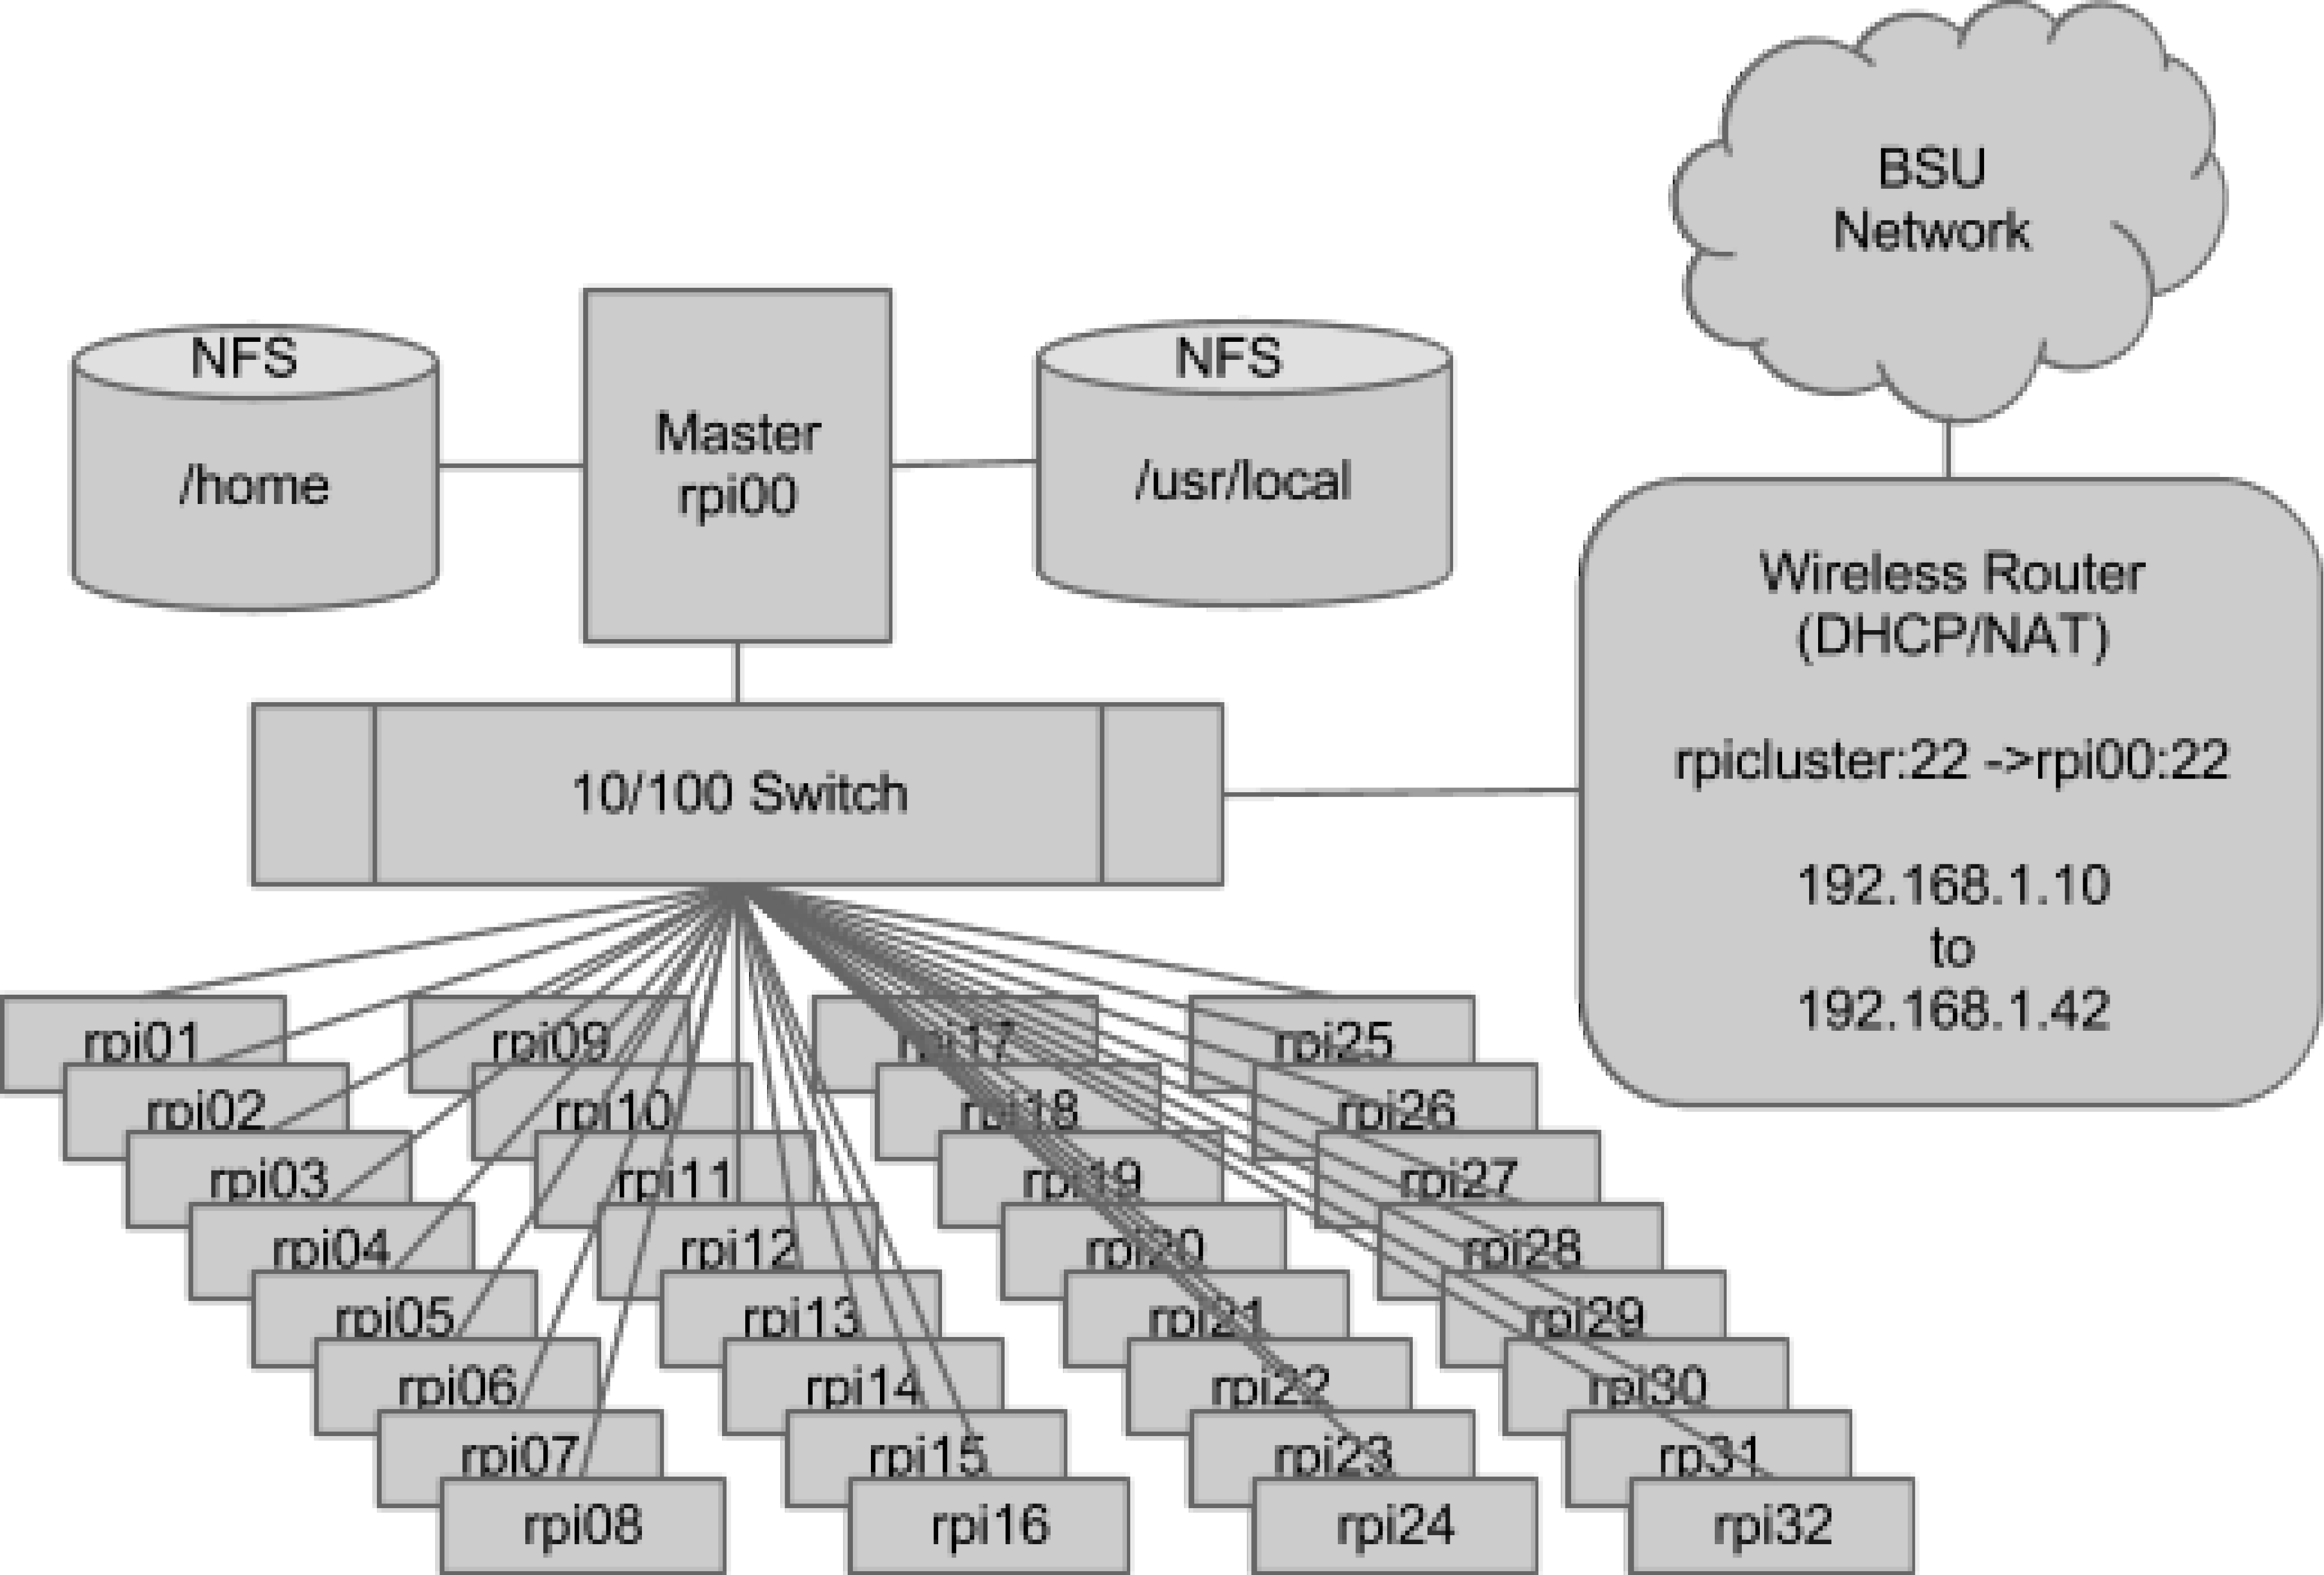
\includegraphics[width=0.4\textwidth]{Chapter1/Figures/kiepert.png}
	\caption[RPiCluster]{Vista general y estructura del sistema (Fuente: Joshua Kiepert)}
	\label{kiepert:structure}
\end{figure}

El coste total del proyecto según Kiepert es de 1967.21 dólares.

\subsection{Dramble (Jeff Geerling)}

El clúster \textit{Dramble} está formado por 6 equipos \textbf{Raspberry Pi} capaces de ejecutar en conjunto el gestor de contenidos \textbf{Drupal}\footnote{\href{https://www.drupal.org/}{drupal.org}}. Es utilizado como servidor de pruebas para la ejecución de instancias de este \textit{software} de forma experimental o durante demostraciones en público\cite{geerlingraspberry}. Se compone del conjunto de nodos \textit{Rasbperry Pi} y los mecanismos de red y alimentación que interconectan y proveen de energía a los mismos.

\begin{figure}[H]
	\centering
	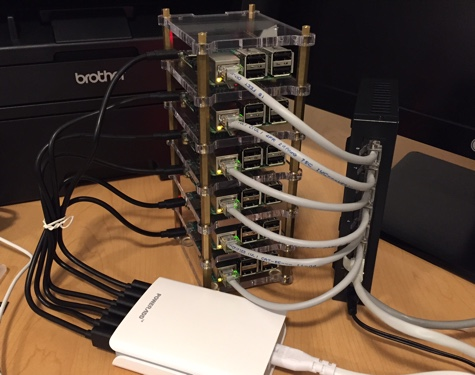
\includegraphics[width=0.5\textwidth]{Chapters/Chapter1/Figures/raspberry-pi-dramble-cluster-wired.jpg}
	\caption[Dramble]{El \textit{Dramble} en ejecución}
	\label{geerling:dramble}
\end{figure}

El coste estimado es de 35 dólares por cada Raspberry Pi mas el coste añadido de la red y el cableado de alimentación, totalizando aproximadamente 300 dólares.

\subsection{Bramble (GCHQ)}

El organismo gubernamental \textit{Government Communication Headquarters}, agencia de inteligencia del Gobierno Británico presentó en la \textit{Big Bang Fair} de 2015 un proyecto educativo que combina 66 \textit{Raspberry Pi} en un clúster jerárquico con 8 grupos de 8 nodos, cada uno de ellos con un coordinador. El cableado se reduce gracias al uso de la tecnología \textbf{PoE} (\textit{Power over Ethernet}), y cada \textbf{Raspberry} cuenta con un conjunto de elementos adicionales, como un reloj de tiempo real, disco duro externo, cámara, o punto de acceso WiFi\cite{gchqbramble}.

\begin{figure}[H]
	\centering
	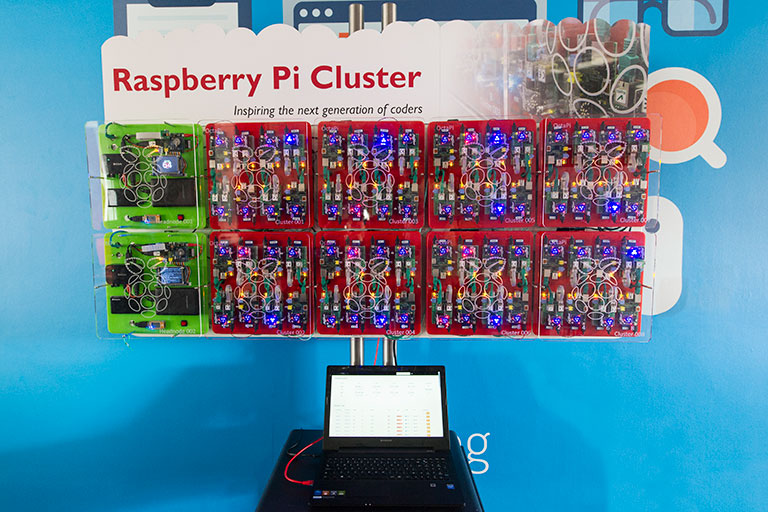
\includegraphics[width=0.8\textwidth]{Chapters/Chapter1/Figures/bramblegchq}
	\caption[Bramble]{Vistazo general de la estructura del sistema Bramble}
	\label{gchq:bramble}
\end{figure}

Se desconocen datos sobre el coste total del sistema.

\subsection{Clúster Iridis (Simon Cox, University of Southampton)}

Con el objetivo de atraer a jóvenes estudiantes al mundo de la computación, el profesor Simon Cox crea este clúster con 64 \textbf{Raspberry Pi B} sobre una estructura construida con LEGO\cite{cox:raspberry}. El sistema está diseñado para ejecutar aplicaciones sobre \textit{MPI}. Se desconocen datos sobre el coste total del sistema.

\begin{figure}[H]
	\centering
	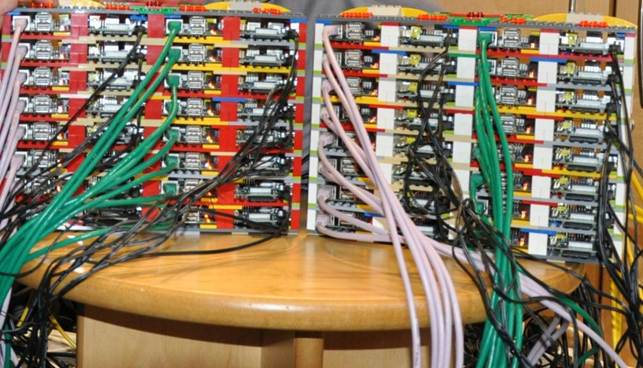
\includegraphics[width=0.65\textwidth]{Chapters/Chapter1/Figures/iridis-pi.jpg}
	\caption[Iridis]{Clúster Iridis}
	\label{cox:iridis}
\end{figure}

\subsection{Paralella}

Paralella es un proyecto de la compañía Adapteva que integra en un único chip un conjunto elevado de procesadores independientes con el objetivo de incrementar la capacidad de procesamiento total del sistema a un coste muy reducido\cite{paralella}. El coste es de 99 dólares por unidad.

\section{Virtualización}

Uno de los mecanismos para crear sistemas distribuidos en auge es la utilización de mecanismos de virtualización (ver \ref{teoria:virtualizacion}, que evitan el uso de diferentes unidades de \textit{hardware}. Estas soluciones se han popularizado en los últimos años principalmente en entornos empresariales, existiendo gran cantidad de proveedores de servicios y herramientas para la creación de un sistema propio (ver \ref{teoria:virtualizacion}). Ejemplos de este tipo de proveedores son \textbf{Amazon Web Services}\footnote{\href{http://aws.amazon.com/}{https://aws.amazon.com}}, \textbf{Google App Engine}\footnote{\href{https://cloud.google.com/appengine/}{https://cloud.google.com/appengine/}}, \textbf{Microsoft Azure}\footnote{\href{http://azure.microsoft.com/}{http://azure.microsoft.com/en-us/}} o \textbf{Digital Ocean}\footnote{\href{http://digitalocean.com}{http://digitalocean.com}}, entre muchos otros. Su éxito reside en su gran versatilidad: es sencillo crear y destruir nuevas réplicas de un sistema bajo demanda, ahorrando costes de forma significativa.

\section{\textit{Commercial Off-The-Shelf hardware}}

Este tipo de hardware está constituido por equipos disponibles al público de forma inmediata (\textit{off the shelf}) y generalmente son máquinas de propósito general, las cuales son interconectadas para crear un sistema distribuido que sirva de alternativa a utilidades más potentes, pero de coste superior (como un \textit{mainframe} o un ordenador de mayor potencia). Su coste económico (que se reduce si existe la posibilidad de aprovechar \textit{hardware} existente en la organización, como equipos de escritorio que no están en uso) es su mayor atractivo.

Un ejemplo de este tipo de sistemas son los clústeres \textit{Beowulf}\cite{beowulf:icpp95}, que se construyen sobre una red de área local y un sistema de intercomunicación como \textbf{MPI}, \textbf{PVM} u \textbf{OpenMP}. Existe gran cantidad de documentación para la creación de un clúster de este tipo\footnote{\href{http://tldp.org/HOWTO/Beowulf-HOWTO/}{tldp.org/HOWTO/Beowulf-HOWTO/}}, así como una serie de recursos (sistemas operativos, herramientas\dots) diseñadas con el propósito específico de crear este tipo de sistemas.